\section{Formalism and details of the modeling}
\label{app:model}

\subsection{Angular Power Spectra}

The angular power spectra for the $\gamma$-ray autocorrelation and for the cross-correlation between the unresolved $\gamma$-ray emission and a galaxy catalog $g$ can be expressed as \cite{camera2013novel,camera2015tomographic,fornengo2014particle}
\begin{eqnarray}
    \label{eq:auto}
     C_\ell^{\gamma \gamma} &=& \int \frac{\de\chi}{\chi^2}\,W_{\gamma}^2(\chi)  
 \,P_{\gamma \gamma}\left(k=\ell/\chi,\chi\right) \\ 
     C_\ell^{\gamma g} &=&\int \frac{\de\chi}{\chi^2}\,W_{\gamma}(\chi)\, W_g(\chi)\,P_{\gamma g}\left(k=\ell/\chi,\chi\right) \; , \label{eq:cross}
 \end{eqnarray}
 where $\ell$ denotes the multipole, $\chi$ is the comoving distance, $W_{\gamma}(\chi)$ and $W_g(\chi)$ are the window functions of the $\gamma$-ray emission and of the galaxy catalog, respectively, that is the functions describing how the observables are distributed in redshift.  $P_{\gamma \gamma}$ and $P_{\gamma g}$ are the 3D power spectra of the auto- and cross- correlation, respectively, which quantify the fluctuations of the corresponding observables. All these components are discussed in the following sub-sections.


\begin{table}[t!]
\centering
\begin{tabular}{|c|cc|}
\hline
Bin & $E_\textrm{{min}}$ & $E_\textrm{{max}}$ \\
\hline
 Low & 8 GeV & 126 GeV \\  
 Mid & 126 GeV & 1.3 Tev \\
 High & 1.3 TeV & 31.6 TeV \\
\hline
  \end{tabular}
\caption{Co-added energy bins used in the analysis for display purposes.}
  \label{Tab:energybin}
\end{table}



$C_\ell^{\gamma \gamma}$ and $C_\ell^{\gamma g}$ are both energy-dependent. In our approach, we compute the correlation functions within the specific energy bins for which the detector sensitivity is available. CTAO sensitivities are provided for 19 energy bins spanning the range (5 GeV, 501 TeV). Due to the sensitivity at low energies, we restrict our analysis to 16  bins, logarithmically spaced within the 30 GeV -- 30 TeV range. For visualization purposes, the energy-dependent quantities are further coadded into 3 broader bins, as summarized in \cref{Tab:energybin}. These low-, medium-, and high-energy bins correspond to the CTAO bin numbers 2-7, 8-12, and 13-18, respectively. However, when computing the DM constraints, we make sure of all 19 energy bins available for CTAO (bins 1 to 19), thereby covering the full energy range from 5 GeV to 501 TeV.

\begin{figure*}[t!]
    \centering
    
\includegraphics[width=0.49\textwidth]{figures/new_analysis/PSF.pdf}
    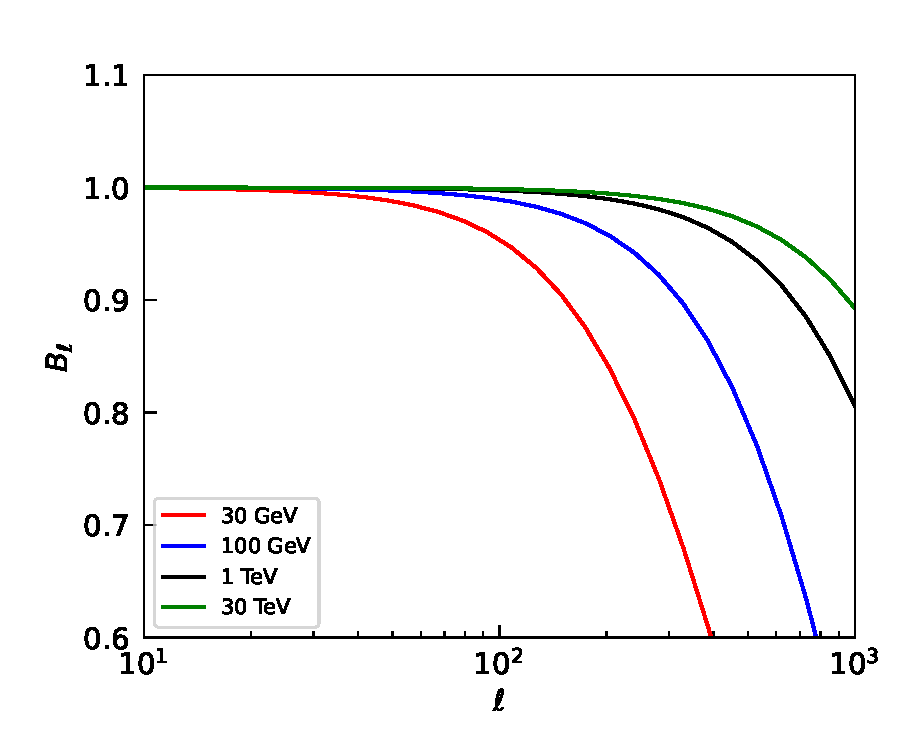
\includegraphics[width=0.49\textwidth]{figures/new_analysis/beam_l.pdf}
    \caption{Left: Point spread functions of CTAO, as a function of angle for different photon energies. Right: The corresponding CTAO beam window functions as a function of multipole.}
    \label{fig:PSF_Beam}
\end{figure*}


The variance of the auto-correlation APS, in the Gaussian approximation, is given by \cref{eq:variance_gammagamma}.

The sky fraction observed by CTAO is $f_\textrm{{sky}} \sim 0.25$ and it is considered energy-independent in our analysis. The beam window functions $B_\ell$ account for the smearing of the angular signal due to the finite angular resolution of the instrument and can be defined in terms of the point spread function (PSF) as 
%
\be
B_\ell(E) = \int \de\theta \, \textrm{{PSF}} (\theta,E) \, \sin \theta \, P_\ell (\cos \theta)\;,
\ee
%
where $P_\ell (\cos \theta)$ are the Legendre Polynomials of order $\ell$. The point-spread function PSF($\theta, E $) has been obtained through a Monte Carlo simulation of the CTAO detector, and is energy-dependent.  \cref{fig:PSF_Beam} shows the PSF($\theta, E$) as a function of the angle $\theta$ (left panel) and the corresponding beam window function as a function of the multipole $\ell$ (right panel) for different energies.


The beam window function in a specific energy bin is then obtained by averaging over the energy-dependent intensity flux $\de I/\de E$, namely
%
\be
\langle B_\ell \rangle = \frac{1}{N}\,\int_\textrm{bin} \de E \, B_\ell(E) \, \frac{\de I}{\de E}\;,
\ee
where $N = \int_\textrm{bin} \de E \, {\de I/\de E}$ For definiteness, we use ${\de I/\de E} \propto E^{-2.3}$, which appropriately matches the observed behavior of the unresolved $\gamma$-ray intensity as measured by \textit{Fermi}-LAT.

%
\begin{figure}[t!]
\centering
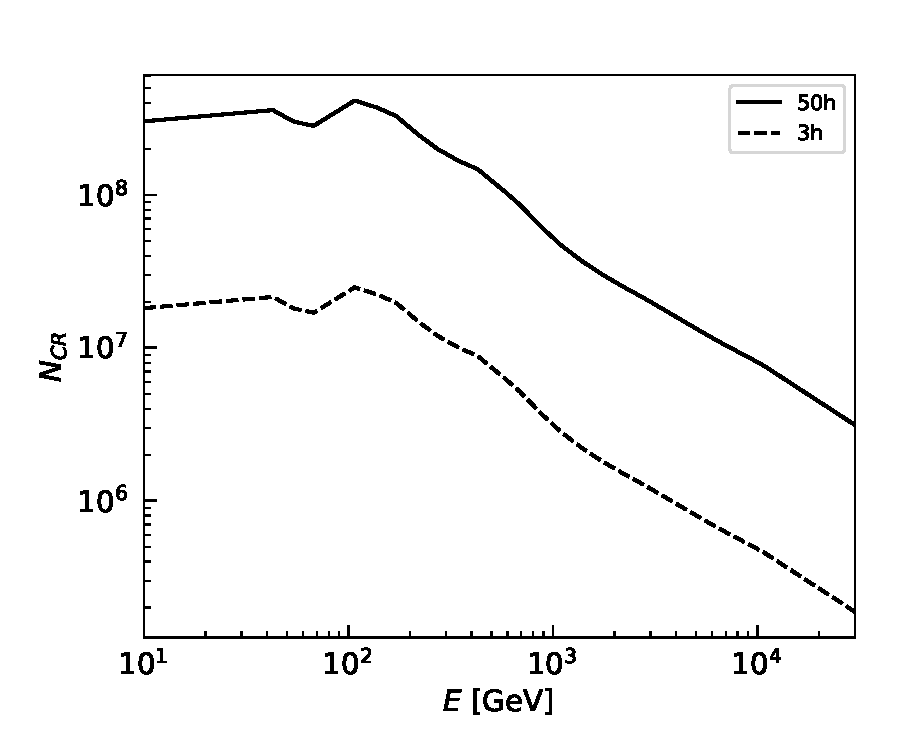
\includegraphics[width=0.49\textwidth]{figures/new_analysis/N_CR.pdf}
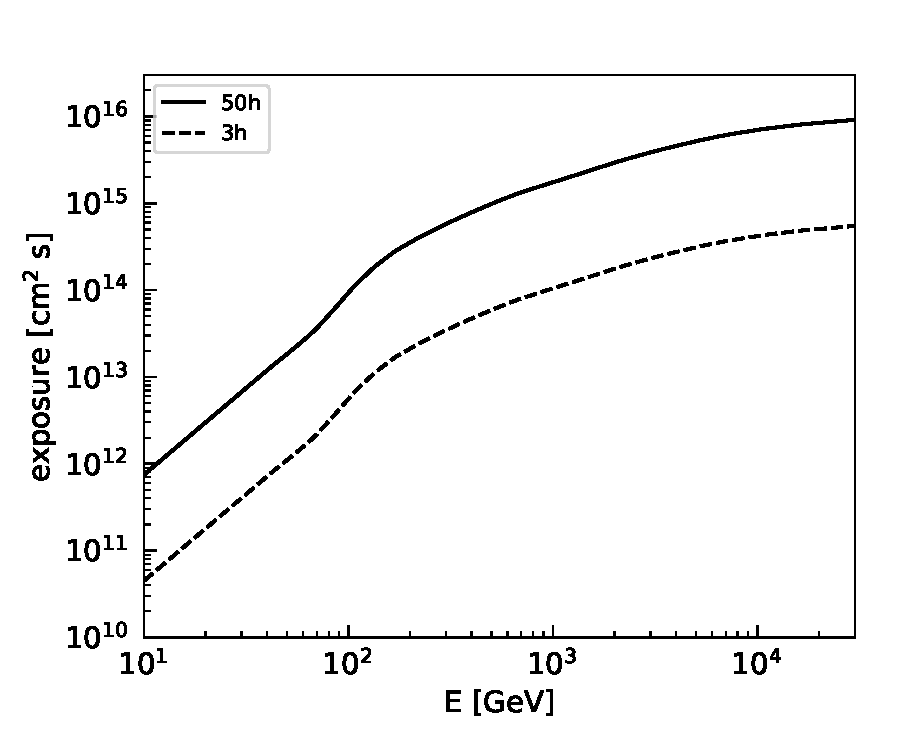
\includegraphics[width=0.49\textwidth]{figures/new_analysis/exposure_CTA.pdf}
\caption{Left: Cosmic-ray background $N_\textrm{{CR}}$ as a function of energy. Right: CTAO exposure as a function of energy.}
\label{noise}
\end{figure}
%

\begin{figure}[t!]
    \centering
    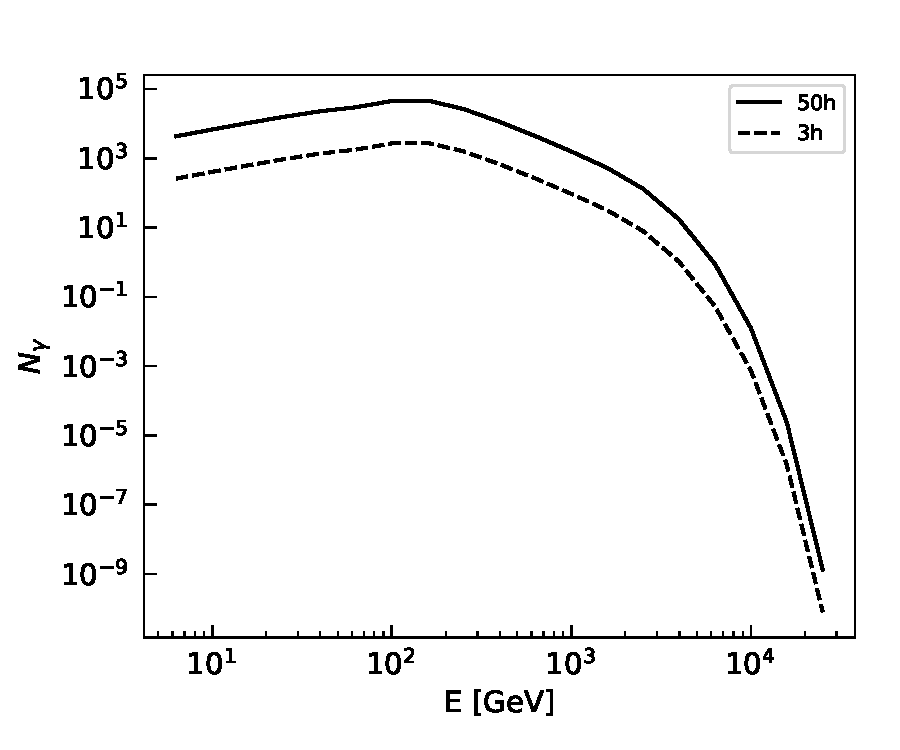
\includegraphics[width=0.45\textwidth]{figures/new_analysis/N_gamma.pdf}
    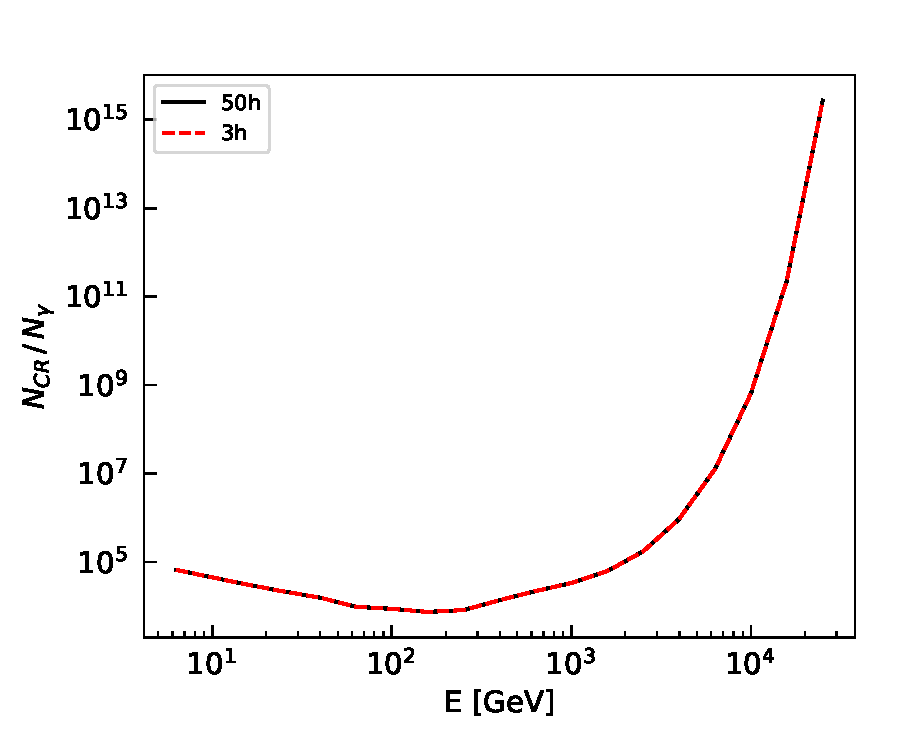
\includegraphics[width=0.45\textwidth]{figures/new_analysis/N_CR_over_N_gamma.pdf}
    \caption{Left: Number of expected $\gamma$-ray events $N_{\gamma}$ in the CTAO survey as a function of energy. Right: Ratio {of cosmic-ray events to expected $\gamma$-ray events ($N_\textrm{CR} / N_{\gamma}$)} after quality cuts in the CTAO survey. The ratio worsens above 1 TeV due to significant $\gamma$-ray suppression from EBL attenuation. $N_\gamma$ is determined for the HSP plus LISP source classes.}
    \label{fig:N_CR_over_N_gamma}
\end{figure}

The photon noise $C_N$ is also energy-dependent and is determined as
\be
C_N = \frac{4\,\pi\,f_\textrm{sky}}{N_\gamma} \left(1 + \frac{N_\textrm{{CR}}}{N_\gamma} \right)\,\langle I \rangle^2\;,
\ee
%
where $N_\textrm{{CR}}$ represents the cosmic-ray irreducible background, $N_\gamma$ is the number of $\gamma$-ray events, and $\langle I \rangle$ denotes the mean $\gamma$-ray intensity in the specific energy bin, which is determined from the window functions as: 
$\langle I \rangle = \int \de\chi \,  W(\chi)$. $N_\gamma$ is therefore related to $\langle I \rangle$ via
\be
N_\gamma = 4\,\pi\,f_\textrm{sky}\,\cal{E}\,\langle I \rangle\;,
\ee
where $\cal{E}$ represents the CTAO exposure in the given energy bin.
The exposure and the counts associated with the cosmic-ray background are derived via Monte Carlo simulations of the CTAO array. The simulation has been performed for 1.62h of observation time, and the results were then rescaled to obtain the exposure for $3\,\textrm{hrs}$ and 50h. \cref{noise} displays the estimated cosmic-ray backgrounds $N_\textrm{{CR}}$ (left panel) and exposures $\cal{E}$ (right panel) as a function of the energy.

 \cref{fig:N_CR_over_N_gamma}  shows the the number of $\gamma$-ray events $N_{\gamma}$ and the  ratio $N_\textrm{{CR}}/N_{\gamma}$ as a function of energy. Since $N_\textrm{{CR}}/N_{\gamma} \gg 1$  in all the energy bins considered in our analysis, the noise can be approximated as
%
\be
C_N \simeq 4\,\pi\,f_\textrm{sky}\,\frac{ N_\textrm{{CR}}}{N_\gamma^2}\,\langle I \rangle^2
\label{CN}
\ee
%
By substituting the expression of $N_\gamma$ in \cref{CN}, it becomes evident that $C_N$ can be expressed only in terms of detector properties and configuration,
%
\be
C_N \simeq \frac{ N_\textrm{{CR}}}{4\,\pi\,f_\textrm{sky} \, \mathcal{E}^2} 
\ee
%
The noise $C_N$ is shown explicitly in \cref{fig:Cl_vs_E}, together with a selection of auto- and cross-correlation energy spectra.


\begin{figure}[t!]
    \centering
    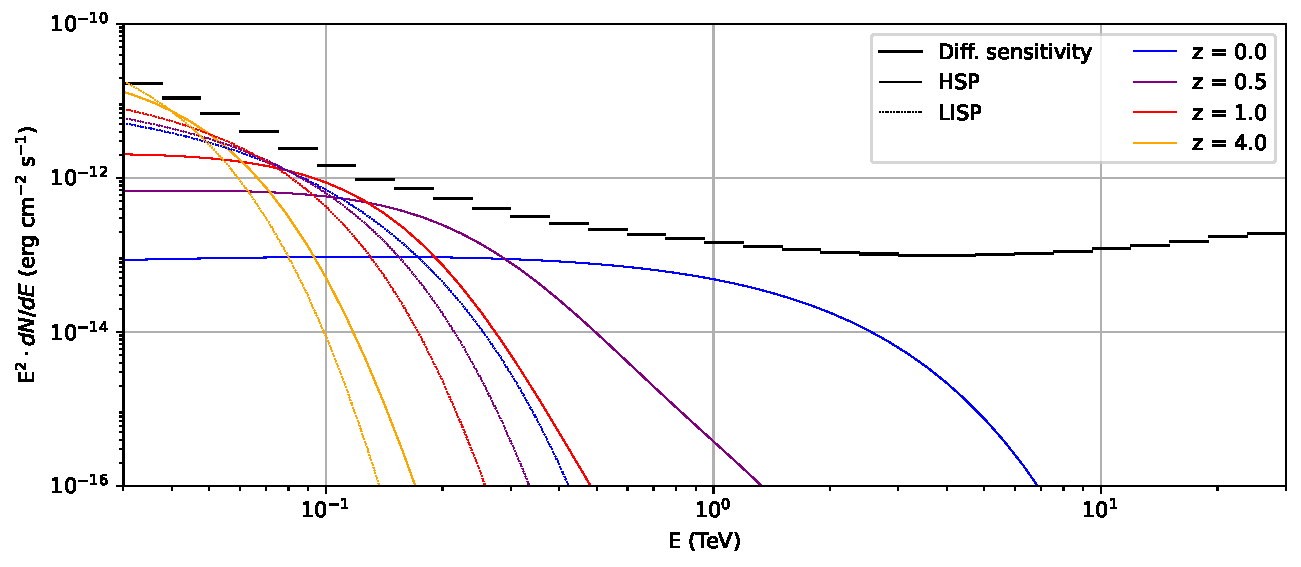
\includegraphics[width=0.9\textwidth]{figures/previous_analysis/integrated_flux_CR+PS_PLEC_rescaleto50h.pdf}
    \caption{Differential flux sensitivity for $5\,\textrm{hrs}$ of observation in the considered CTAO energy range (thick black horizontal dashes), compared with the energy spectra of HSP and LISP sources (solid and dotted lines, respectively) at four different redshifts. The spectra are normalized to the minimal flux detectable with the planned EGAL survey.}
    \label{fig:diffsens}
\end{figure}

In the case of cross-correlations, the variance is instead given by \cite{camera2013novel,camera2015tomographic,fornengo2014particle}
\begin{equation}
    (\varDelta C^{\gamma g}_\ell)^2 = \frac{1}{\left(2\ell+1 \right) f_\textrm{{sky}}} \left[(C_\ell^{\gamma g})^2 + \left(C_\ell^{\gamma \gamma} + \frac{C_N}{B_\ell^2}\right)\left(C_\ell^{gg} + C_{N_g} \right) \right].
    \label{eq:deltagamma g}
\end{equation}
where $C_\ell^{gg}$ is the galaxy auto-correlation, $C_N$ is the same as in the auto-correlation case, $C_{N_g}$ is the galaxy catalog noise. There is no beam correction in the galaxy term, as the angular resolution on the galaxy catalog is on the order of arcseconds,  making it negligible in this analysis. The galaxy noise is given by
\be
C_{N_g}= \frac{4\,\pi\,f_{\textrm{sky},g}}{N_g}
\ee
where $f_{\textrm{sky},g}$ represents the fraction of the sky covered by the catalog, and $N_g$ is the number of galaxies in the catalog. \cref{fig:Cl_vs_E} shows the quantity $\sqrt{C_N\,C_{N_g}}$ as a representative level for the cross-correlation noise, which approximately corresponds to the noise expected in a noise-dominated regime. 

\subsection{Window functions}
\label{app:window}

\subsubsection{Gamma-ray astrophysical sources}
\label{app:Wastro}

The window function for the $\gamma$-ray emission of unresolved astrophysical sources can be written as
\begin{equation}
    W(E, \chi) =  \frac{\de W}{\de E\,\de\chi} = \frac{d_L^2(z)}{\left(1+z \right)^2} \; \int_{L_\textrm{min}}^{L_\textrm{th}(z)} \;  \de L \; \varPhi(L,z) \, \frac{d F}{d E}(E,L,z) \, \exp[-\tau(E,z)] 
    \label{eq:window_astro}
\end{equation}
where $d_L(z)$ is the luminosity distance, $\varPhi(L,z)$ is the $\gamma$-ray luminosity function of the source population. In the present analysis, we use the luminosity functions of HSP and LISP as reported in \cite{DiMauro:2013zfa}.
Note that the above window function, which is used in Eq.\ref{eq:auto}-\ref{eq:cross} is differential in comoving distance, $\chi$. The analogous quantity differential, differential in $z$, would be $W(E,z)=\frac{\de W}{\de E\,\de z} = \frac{\de W}{\de E\,\de\chi} \frac{\de\chi}{\de z} = W(E,\chi) \frac{\de\chi}{\de z}$ where $\frac{\de\chi}{\de z} = \frac{c}{H(z)}$. Also note that the above window is differential in energy. In Eq. \ref{eq:auto}-\ref{eq:cross}, however, the corresponding quantity must be integrated over the energy bin considered. $L$ is the $\gamma$-ray luminosity of the source, conventionally integrated over the interval (0.1, 100) GeV, that is
\be
L = \int_{0.1\, \textrm{GeV}}^{100\, \textrm{GeV}} \de E_r \, \frac{\de L}{\de E_r}
\ee
where $E_r$ is the source rest-frame energy, related to the observed energy by $E_r = (1+z) E$, and $\de F/\de E$ is the spectral energy distribution (SED) of the sources, which we model as a power law with index $\varGamma$ and an exponential cutoff,
\begin{equation}
\frac{\de F}{\de E} = A(L,z) \; E^{-\varGamma} \, \exp(-E/E_\textrm{cut})
\label{eq:SED}
\end{equation}
The values of $\varGamma$ and $E_\textrm{cut}$ for the two classes of astrophysical sources adopted in our models are reported in \cref{table:BLLACS}, together with the minimum luminosity of the source classes $L_\textrm{min}$. The parameter $A$, on the other hand, can be related to the luminosity $L$, by observing that (see Eq.\ 22 in \cite{Hogg:1999ad})
\be
L = \frac{4\,\pi\,d_L^2(z)}{(1+z)} \int_{0.1\, \textrm{GeV}}^{100\, \textrm{GeV}} \de E_r \, E_r \, \frac{\de F}{\de E_r} = 4\,\pi\,d_L^2(z) \int_{0.1\, \textrm{GeV}/(1+z)}^{100\, \textrm{GeV}/(1+z)} \de E \, E \, \frac{\de F}{\de E}
\label{eq:luminosity}
\ee
and therefore:
\be
A(L,z) = \frac{L}{4\,\pi\,d_L(z)^2} 
\left[ 
\int_{0.1\, \textrm{GeV}/(1+z)}^{100\, \textrm{GeV}/(1+z)} 
\de E \,  E^{(-\varGamma + 1)} \, \exp(-E/E_\textrm{cut}) \right]^{-1}
\ee


The last term in \cref{eq:window_astro} models the $\gamma$-ray absorption on extragalactic background light (EBL). For the optical depth $\tau(E,z)$, we adopt the results from Ref. \cite{Finke:2009xi}. The maximal luminosity $L_\textrm{th}(z)$ in \cref{eq:window_astro}, which refers to the threshold of detectability of resolved sources by the detector, depends on the CTAO sensitivity $F_\textrm{sens}^\textrm{CTA}(z)$ to point sources in the energy range of operation, which in our analysis is defined as (30 GeV, 30 TeV) 
\be
F_\textrm{sens}^\textrm{CTA}(z) = \int_{30\, \textrm{GeV}}^{30\, \textrm{TeV}} \de E \, \frac{\de F}{\de E} \, \exp[-\tau(E,z)] = 
A_\textrm{th}(z)\; \int_{30\, \textrm{GeV}}^{30\, \textrm{TeV}} \, \de E \, E^{-\varGamma} \, \exp(-E/E_\textrm{cut}) \exp[-\tau(E,z)]
\label{FsensCTA}
\ee
From $F_\textrm{sens}^\textrm{CTA}(z)$, it is therefore possible to determine the value of $A_\textrm{th}(z)$, which allows us to determine the threshold luminosity by means of \cref{eq:luminosity} as
%
\be
L_\textrm{th}(z) = 4\,\pi\,d_L^2(z) \; F_\textrm{sens}^\textrm{CTA}(z) \; 
\frac{
\int_{0.1\, \textrm{GeV}/(1+z)}^{100\, \textrm{GeV}/(1+z)} \de E \, E^{-\varGamma+1} \, \exp(-E/E_\textrm{cut})}
{\int_{30\, \textrm{GeV}}^{30\, \textrm{TeV}} \, \de E \, E^{-\varGamma} \, \exp(-E/E_\textrm{cut}) \exp[-\tau(E,z)]}
\label{eq:threshold}
\ee
%

The HSP and LISP point source sensitivity has been obtained through extensive Monte Carlo simulations \cite{CTAConsortium:2018tzg,VeronikaThesis} and is shown in \cref{fig:diffsens} for $3\,\textrm{hrs}$ of observation across different energy bins. The same plot compares the differential sensitivity with the $\gamma$-ray spectra of LISP and HSP blazars normalized to the minimum detectable intensity. As shown, the spectra observed at Earth are redshift-dependent, as sources at different redshifts experience different levels of EBL absorption. \cref{fig:Fsens} instead shows the integrated HSP and LISP point source sensitivity in the energy range 30 GeV to 30 TeV as a function of $z$, where the normalization of the SED in \cref{eq:SED} has been fixed to its threshold value $A_\textrm{th}(z)$, obtained from \cref{FsensCTA} by employing the Monte Carlo modeling of $F_\textrm{sens}^\textrm{CTA}(z)$.


\begin{figure}[t!]
    \centering
    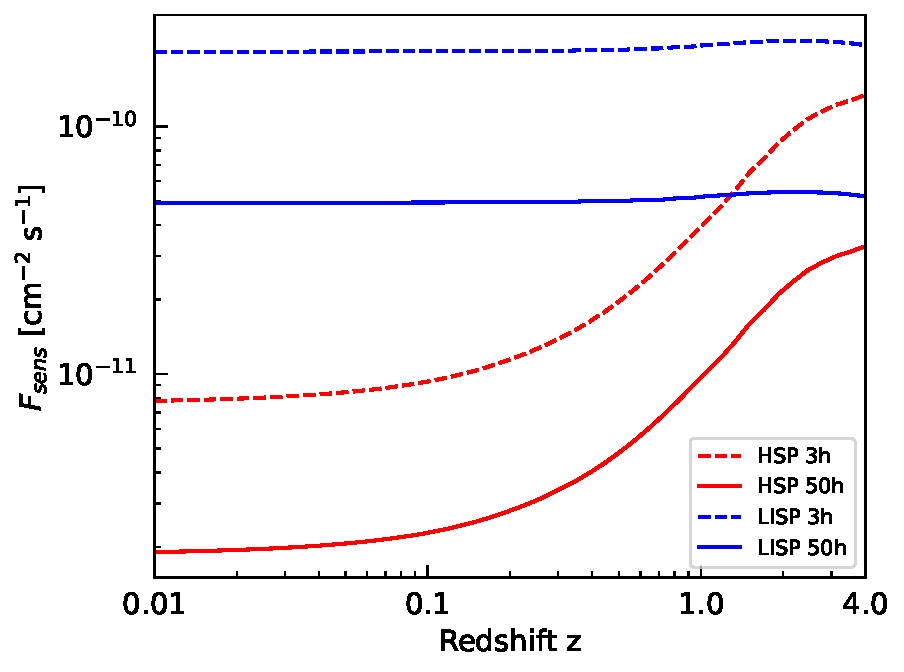
\includegraphics[width=0.45\textwidth]{figures/new_analysis/Fsens.pdf}
    \caption{CTA sensitivity $F_\textrm{sens}^\textrm{CTA}(z)$ for $3\,\textrm{hrs}$ and $5\,\textrm{hrs}$ of observation as a function of redshift, for the HSP and LISP $\gamma$-ray source classes.}
    \label{fig:Fsens}
\end{figure}


\subsubsection{Gamma-ray emission from dark matter}
\label{app:WDM}

Window functions for dark matter are modeled as in Refs. \cite{camera2015tomographic,fornengo2014particle,Cuoco:2015rfa}, to which we refer for additional details. For decaying dark matter, we have
%
 \be
     W(E, \chi) = \frac{\de W}{\de E\,\de\chi} = \, \left (\frac{\varOmega_\textrm{DM} \,\rho_\textrm{c} }{m_{\chi}} \right) \, \frac{\varGamma_\textrm{d}}{4 \pi}  \frac{\de N}{\de E}[(1+z)/E] \, \exp[-\tau(E,z)]
     \label{eqn:Wdec}
 \ee
%
where $\varOmega_\textrm{DM}$ is the dark matter density parameter, $\rho_\textrm{c}$ is the critical density of the Universe,
$m_{\chi}$ the DM particle mass, $\varGamma_\textrm{d}$ the DM decay rate, $dN/\de E$ the $\gamma$-ray energy spectrum per decay event, which we take from \cite{Arina:2023eic} for decay into $b\bar{b}$, $\tau^+ \tau^-$, $W^+ W^-$. The last term in the equation refers again to $\gamma$-ray absorption, as discussed for the astrophysical sources.


For annihilating DM, the window function reads
%
 \be
     W(E, \chi) = \frac{\de W}{\de E\de\chi} = \frac{1}{4 \pi} \, \frac{\langle \sigma v \rangle}{2} \varDelta^2(z) \, \left (\frac{\varOmega_\textrm{DM} \,\rho_\textrm{c} }{m_{\chi}} \right)^2 (1+z)^3  \frac{d N}{d E}[(1+z)E]  \exp[-\tau(E,z)]\;,
     \label{eqn:Wann}
 \ee
%
where  $\langle \sigma v \rangle$ is the velocity-averaged annihilation cross-section. Unlike DM decay, the annihilation window function also contains the flux multiplier factor $\varDelta^2(z)$, which accounts for the enhancement of the flux due to the clumping of DM and the presence of sub-structures within the DM halos. Details on the way we model the flux multiplier can be found in Ref. \cite{Pinetti:2021jjs,Pinetti:2019ztr,Arcari:2022zul}.
Window functions for both DM and astrophysical sources are plotted in Fig.\ref{fig:zWindows} as a function of redshift for two different energies, and for $3\,\textrm{hrs}$ and $5\,\textrm{hrs}$ of observation time. It can be seen that the DM window always peaks at low $z$, while the astrophysical signal peaks at $z\sim 0.4-0.5$ at 50 GeV and  $z\sim 0.1-0.2$ at 1 TeV, with the horizon shrinking due to the effect of EBL $\gamma$-ray absorption.
\cref{fig:E2_mean_intensity}, instead, displays the intensity $\langle I \rangle$ as a function of the energy for the two classes of astrophysical sources used in the analysis and for a few representative cases of DM annihilation. 


\subsubsection{Galaxy Catalogs}
\label{app:Wgal}

The galaxy-catalog window functions are given by the redshift distribution of the number of objects in the catalog, namely
\begin{equation}
      W_g(z) = \frac{\de N_g}{\de z}\;.
\end{equation}
 The window function is normalized such that $\int \de z \, W_g(z) = 1$. Note again that $W_g(\chi)$ entering the cross-correlation APS is related to the redshift-dependent window function as $W_g(\chi) = W_g(z) \frac{\de z}{\de\chi} = W_g(z) H(z)/c$, where $H(z)$ is the Hubble parameter and $c$ the speed of light.
 In this way we also have  $\int \de\chi \, W_g(\chi) = 1$.
We use the $dN_g/\de z$ as given in \cite{Huchra:2011ii,Ando:2017wff} for 2MRS and \cite{2MASS:2006qir,Bilicki:2013sza} for 2MASS.



\begin{figure}[t!]
    \centering
    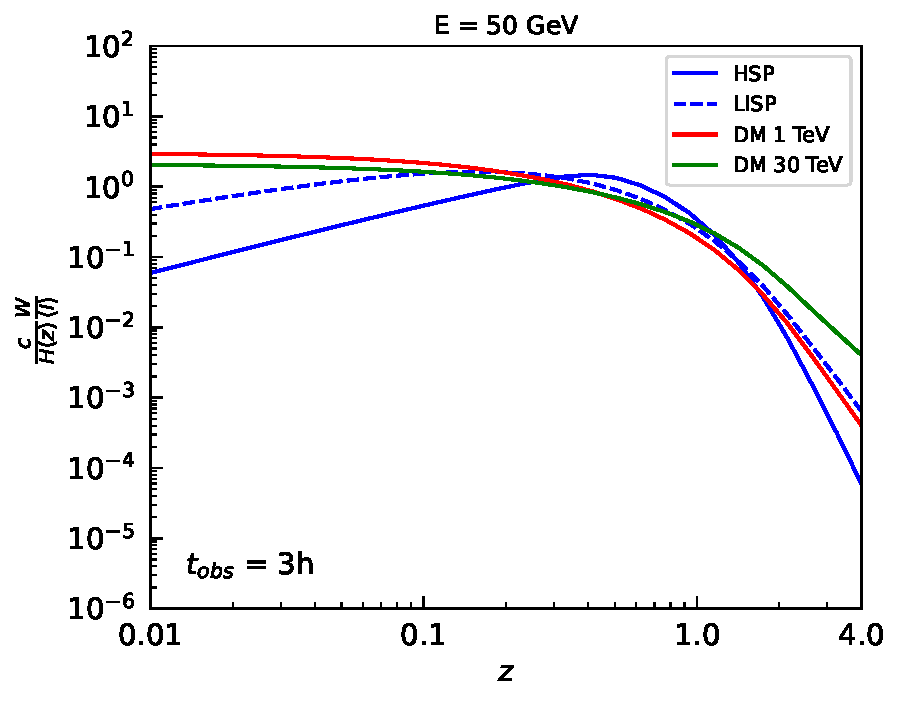
\includegraphics[width=0.45\textwidth]{figures/new_analysis/W_at_50GeV_3h.pdf}
    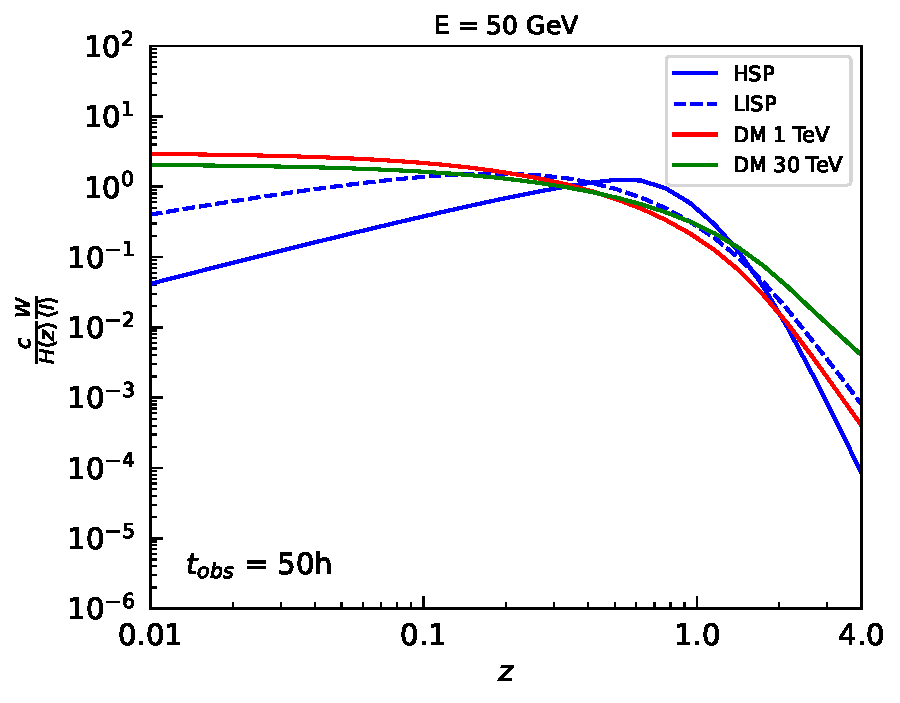
\includegraphics[width=0.45\textwidth]{figures/new_analysis/W_at_50GeV_50h.pdf}
    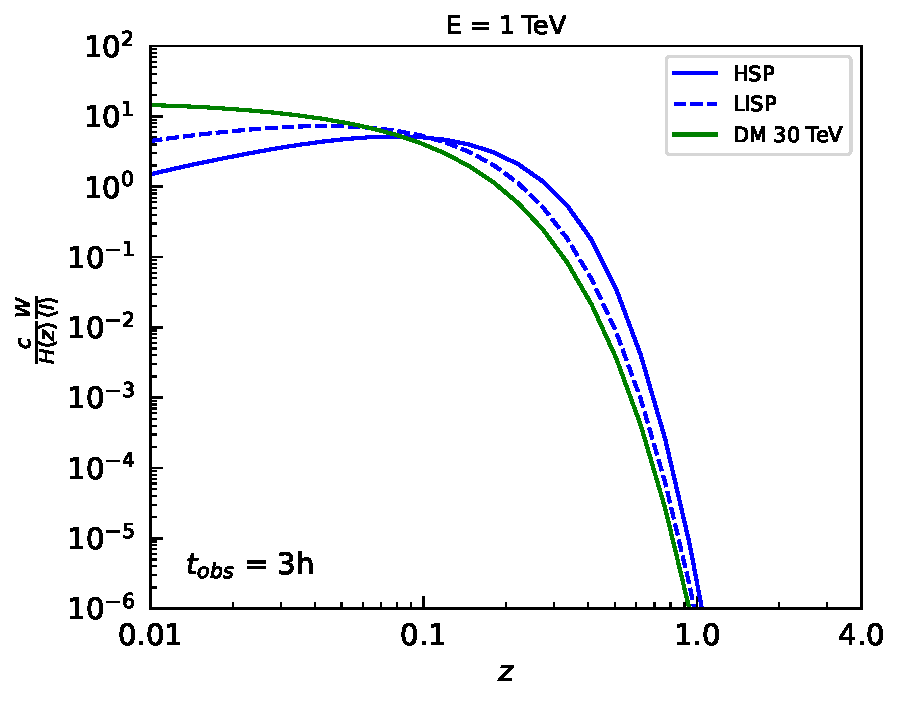
\includegraphics[width=0.45\textwidth]{figures/new_analysis/W_at_1TeV_3h.pdf}
    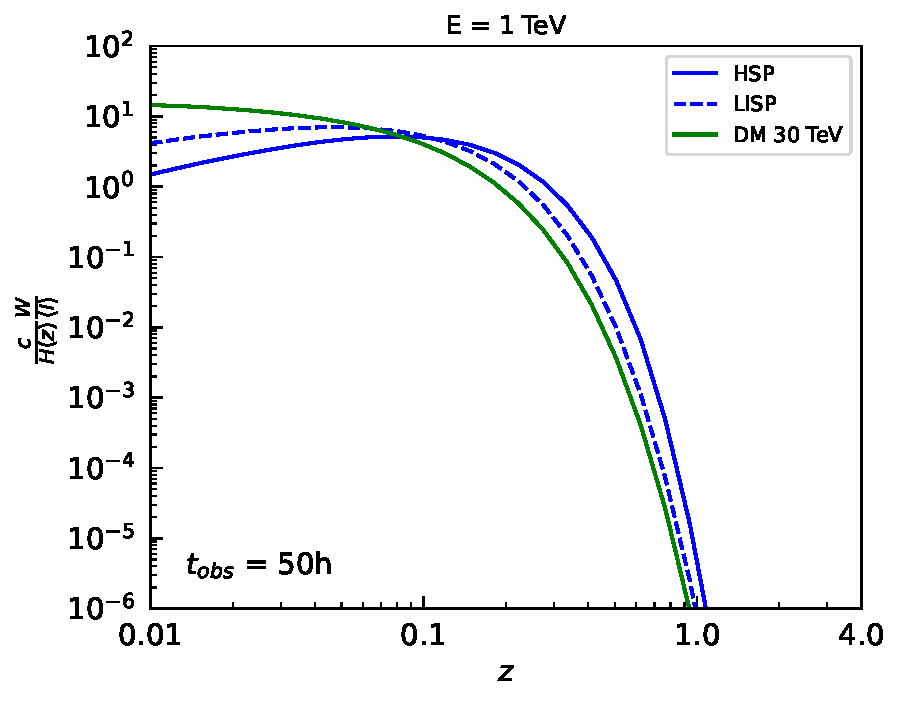
\includegraphics[width=0.45\textwidth]{figures/new_analysis/W_at_1TeV_50h.pdf}
    \caption{$\gamma$-ray window functions, normalized to the mean $\gamma$-ray intensity, as a function of redshift (and divided by the Hubble parameter). Left panels show results for 3 hours of observation, and right panels for 50 hours. The blue solid and dashed lines represent the HSP and LISP astrophysical sources, respectively. The red and green solid lines refer to DM annihilation into $b\bar{b}$, $\langle \sigma v \rangle = 3 \times 10^{-26}$cm$^{-3}$s$^{-1}$ and masses of 1 TeV (red) and 30 TeV (green). The upper row is calculated for a $\gamma$-ray energy of 50 GeV, while the lower row is for 1 TeV (only the 30 TeV DM case is shown here). {The 3-hour observation time cases are the same as shown in Fig. \ref{fig:window_main}}.}
    \label{fig:zWindows}
\end{figure}


\begin{figure}[t!]
    \centering
    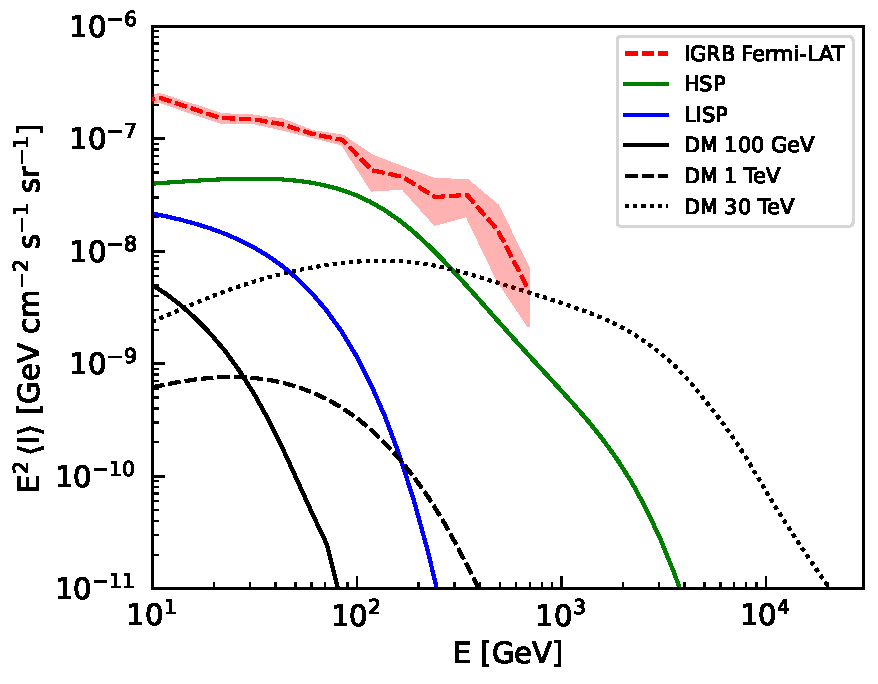
\includegraphics[width=0.45\textwidth]{figures/new_analysis/E2_mean_intensity.pdf}
    \caption{$\gamma$-ray intensity in our benchmark model for HSP (solid green) and LISP (solid blue), along with three cases of dark matter annihilation for particle masses of 100 GeV (solid black), 1 TeV (dashed black). and 30 TeV (dotted black). The 100 GeV and 1 TeV lines correspond to an annihilation cross-section $\langle \sigma v \rangle = 3 \times 10^{-26}$cm$^{-3}$s$^{-1}$, while for 30 TeV we adopted $\langle \sigma v \rangle = 3 \times 10^{-23}$cm$^{-3}$s$^{-1}$. The figure also shows the measured IGRB (red dashed line and red band for its uncertainty) \cite{Ackermann_2015}.}
    \label{fig:E2_mean_intensity}
\end{figure}


\subsection{Galaxies Halo Occupation Distribution}
To model the clustering of galaxies within the catalog, we use the Halo Occupation Distribution (HOD) formalism (see  \cite{Zheng:2004id,Berlind:2001xk,Cooray:2002dia}).


The number of galaxies residing within a DM halo of mass $M$ is parameterized as
\begin{eqnarray}
\langle N_\textrm{cen}(M)\rangle &=& \frac{1}{2}\left[1+\textrm{erf}\left(\frac{\log M-\log M_\textrm{th}}{\sigma_\textrm{logM}}\right)\right]\;, \label{eq:HOD1}\\
\langle N_\textrm{sat}(M)\rangle &=& \left( \frac{M}{M_1} \right)^\alpha \exp{\left(-\frac{M_\textrm{cut}}{M}\right)}\;,\label{eq:HOD2}
\end{eqnarray}
where, for a halo of mass $M$, $\langle N_\textrm{cen}(M) \rangle$ is the average number of galaxies at the center of the halo and $\langle N_\textrm{sat}(M)\rangle$ represents the average number of satellite galaxies.
The parameters $M_\textrm{th}, \ \sigma_\textrm{logM}, \ \alpha, \ M_1, \ M_\textrm{cut}$ characterize the HOD and we chose them according to 
\cite{Ando:2017wff} for 2MRS and \cite{Cuoco:2015rfa} for 2MASS.



\subsection{3D Power Spectra}
The 3D Power Spectra $P(k)$  (PS) have been calculated by using the Halo Model formalism \cite{Cooray:2002dia}. We have derived the autocorrelation 3D PS of decaying DM $P_\delta(k)$, annihilating DM $P_{\delta^2}(k)$ and astrophysical sources $P_\gamma(k)$, and the 3D cross-correlation PS among the same three categories of tracers: $P_{g\delta}(k)$ for the cross-correlation between galaxies and decaying DM $\gamma$-ray emission,  $P_{g\delta^2}(k)$ for the cross-correlation between galaxies and annihilating DM $\gamma$-ray emission, for the cross-correlation between galaxies and astrophysical sources $\gamma$-ray emission $P_{g\gamma}(k)$. The explicit formulas for the power spectra are reported in Ref. \cite{Cuoco:2015rfa}, to which we refer the reader for details. 

Figs. \ref{fig:PS_tot}-\ref{fig:P1h_P2h} report the plots of the various 3D power spectra adopted in the analysis. Figs.\ref{fig:Cl_1TeV_binned}-\ref{fig:Cl_1TeV_cross} show a few samples of auto and cross-correlation APS as a function of the multipole $\ell$. It can be seen that auto APS of astrophysical sources is constant in $\ell$, since they are point-like, while the DM APS presents some structure due to the extension of the DM halos. Fig.\ref{fig:Cl_vs_E}, instead, shows the APS as a function of energy at a fixed multipole $\ell=100$. For comparison, the auto- and cross-correlation noise level is plotted, thus showing that the expected signal-to-noise ratio is typically low.



\begin{figure}[t!]
    \centering
    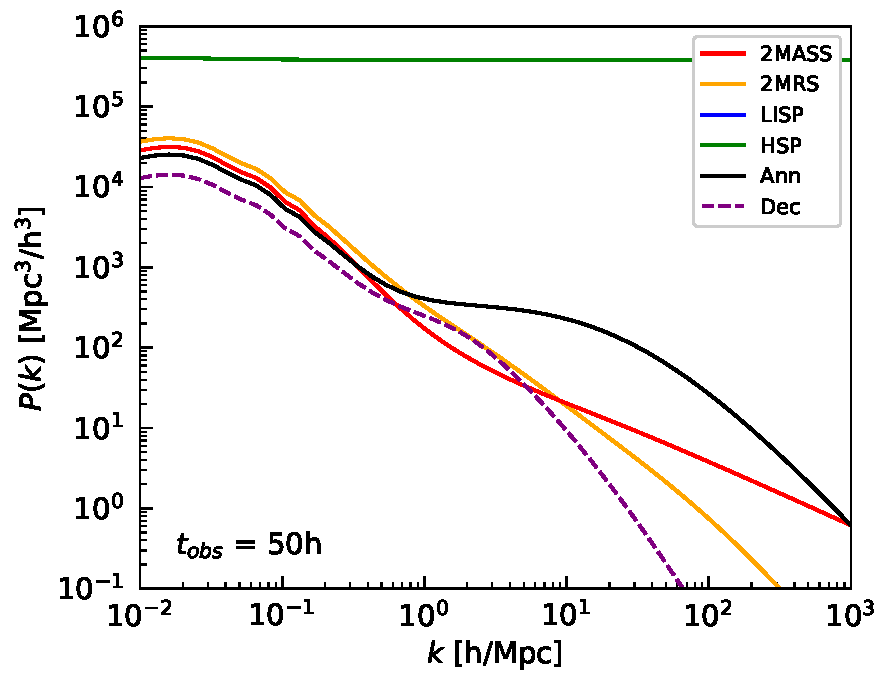
\includegraphics[width=0.45\textwidth]{figures/new_analysis/PS_auto_vs_k_tot.pdf}
    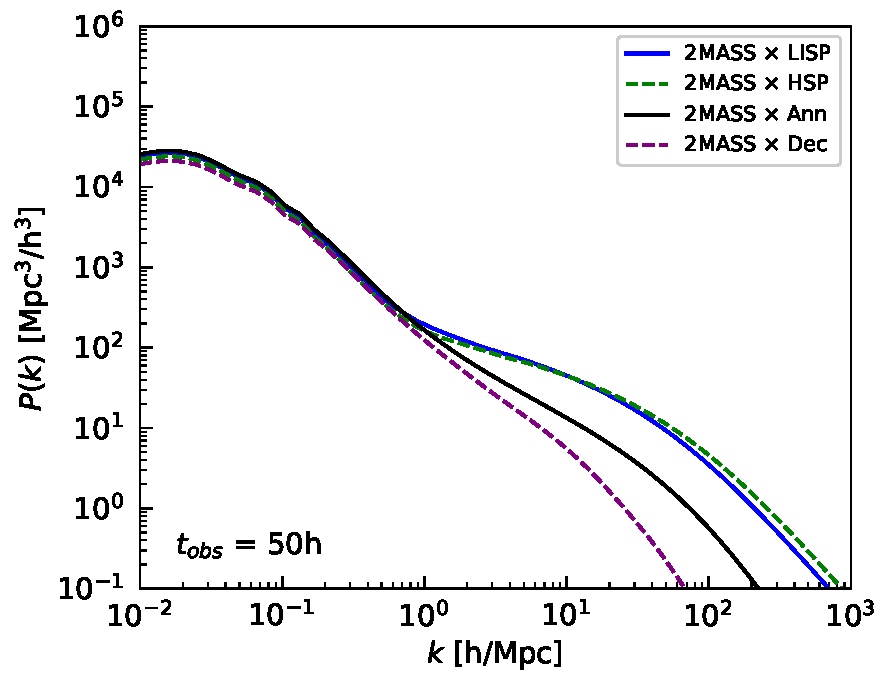
\includegraphics[width=0.45\textwidth]{figures/new_analysis/PS_cross_vs_k_tot.pdf}
    \caption{Left: Auto-correlation 3D power spectra for 2MASS and 2MRS galaxies, LISP and HSP astrophysical sources, and annihilating and decaying dark matter. Right: Cross-correlation 3D power spectra for the cross-correlation between 2MASS galaxies and the various $\gamma$-ray source types considered in our analysis: LISP, HSP, annihilating and decaying dark matter.}
    \label{fig:PS_tot}
\end{figure}

\begin{figure}[t!]
    \centering
    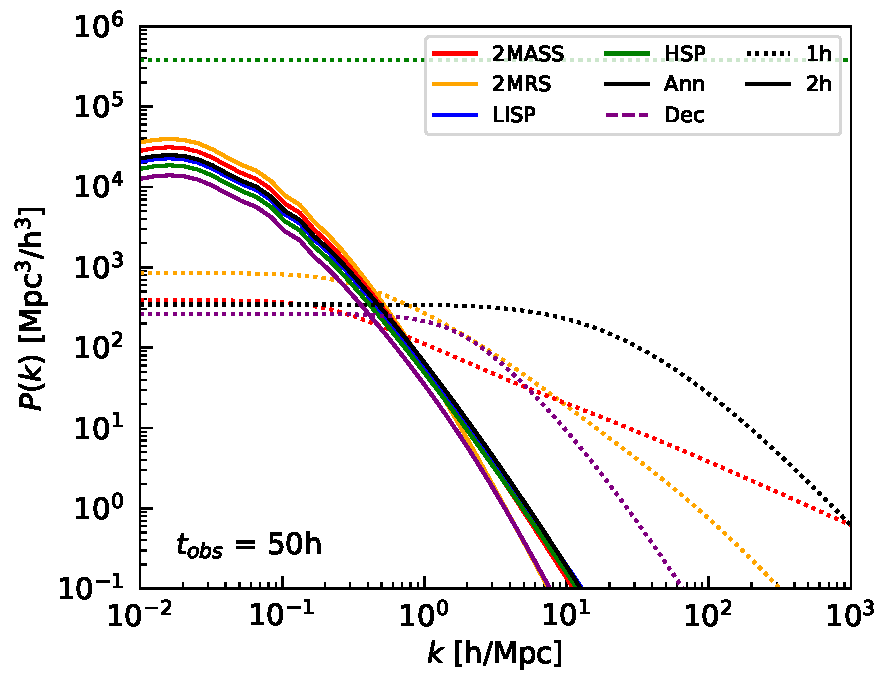
\includegraphics[width=0.45\textwidth]{figures/new_analysis/PS_auto_vs_k.pdf}
    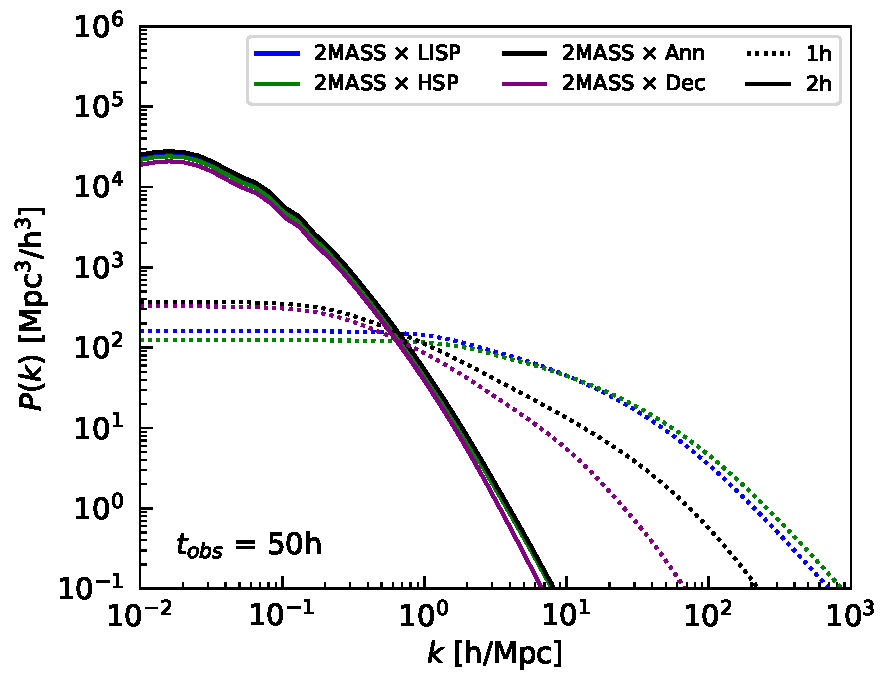
\includegraphics[width=0.45\textwidth]{figures/new_analysis/PS_cross_vs_k.pdf}
    \caption{The same as Fig.\ref{fig:PS_tot} but with the 1-halo (dotted) and the 2-halo (solid) terms shown separately. }
    \label{fig:P1h_P2h}
\end{figure}


\begin{figure}[t!]
    \centering
    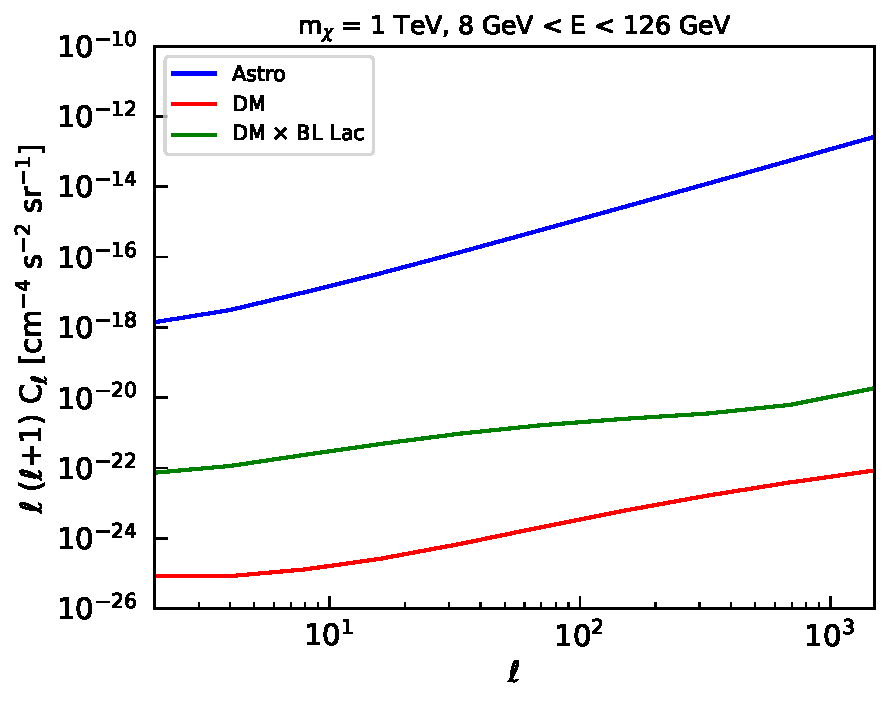
\includegraphics[width=0.45\textwidth]{figures/new_analysis/Cl_1TeV_low_7bin_ell.pdf}
    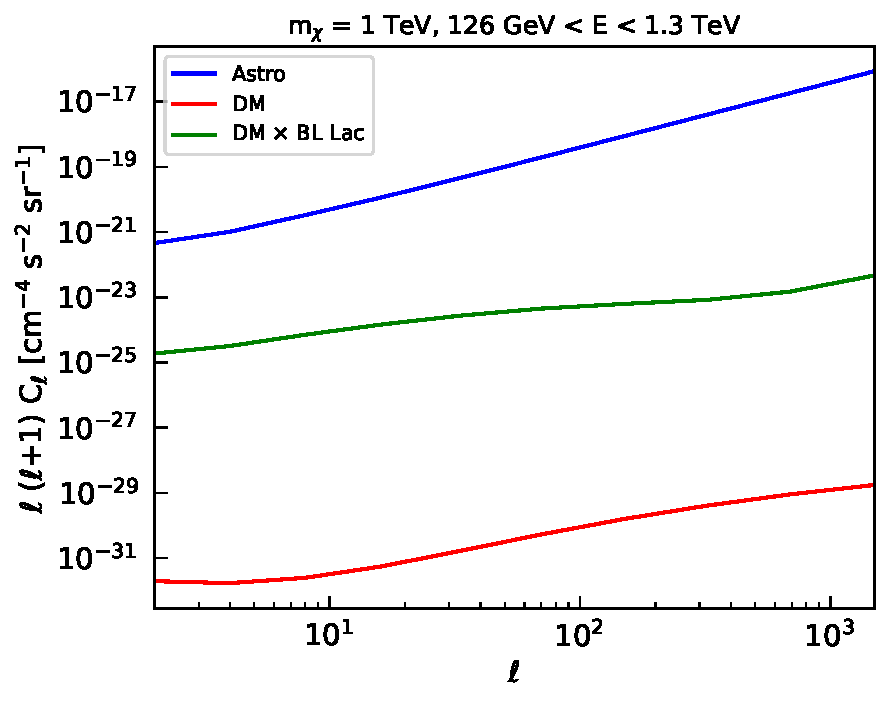
\includegraphics[width=0.45\textwidth]{figures/new_analysis/Cl_1TeV_mid_7bin_ell.pdf}
    \caption{Angular power spectra of the $\gamma$-ray auto-correlation as a function of the multipole, for two different energy bins. The upper (blue) curve refers to the auto-correlation among astrophysical sources, the median (green) and lower (red) curves to the correlation between sources and dark matter and the autocorrelation of dark matter, respectively, for a dark matter mass of 1 TeV and annihilation into $b\bar{b}$ with a cross-section $\langle \sigma v \rangle = 3 \times 10^{-26}$cm$^{-3}$s$^{-1}$.}
    \label{fig:Cl_1TeV_binned}
\end{figure}

\begin{figure}[t!]
    \centering
    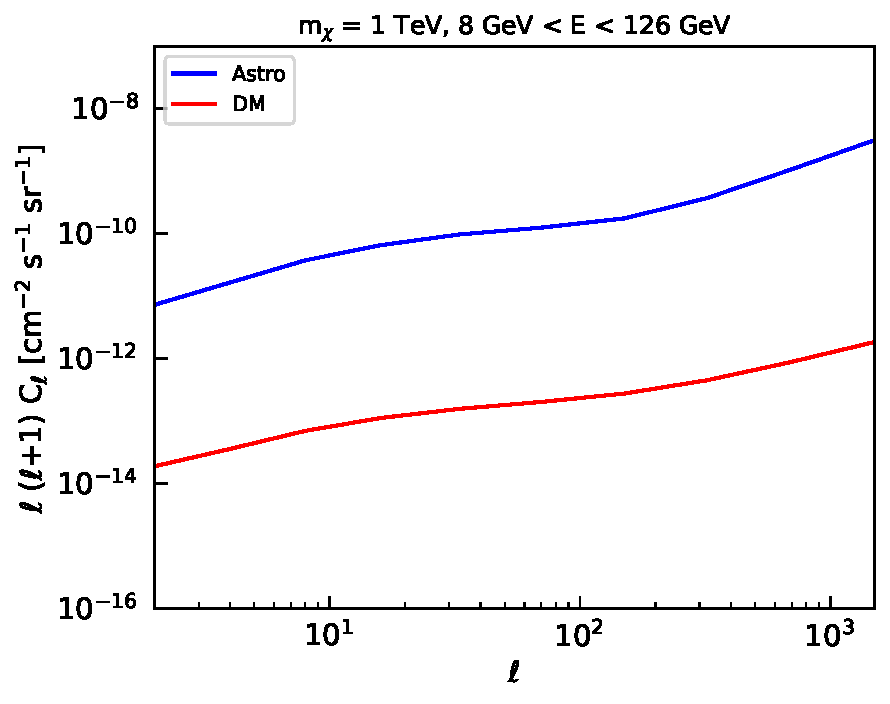
\includegraphics[width=0.45\textwidth]{figures/new_analysis/Cl_1TeV_low_7bin_ell_cross.pdf}
    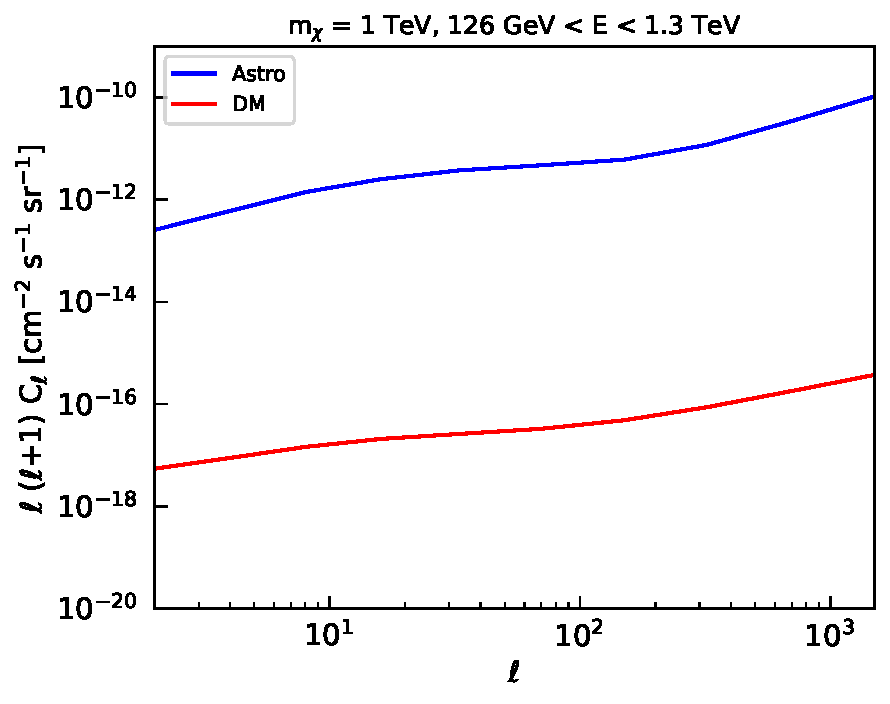
\includegraphics[width=0.45\textwidth]{figures/new_analysis/Cl_1TeV_mid_7bin_ell_cross.pdf}
    \caption{Angular power spectra of the $\gamma$-ray cross-correlation with 2MASS galaxies, as a function of the multipole, for two different energy bins. The upper (blue) curve refers to the cross-correlation with astrophysical sources, while the lower (red) curves represent the correlation with a dark matter signal produced by a particle with mass of 1 TeV and annihilation cross-section into $b\bar{b}$ of $\langle \sigma v \rangle = 3 \times 10^{-26}$cm$^{-3}$s$^{-1}$.}
    \label{fig:Cl_1TeV_cross}
\end{figure}

\begin{figure}[t!]
    \centering
    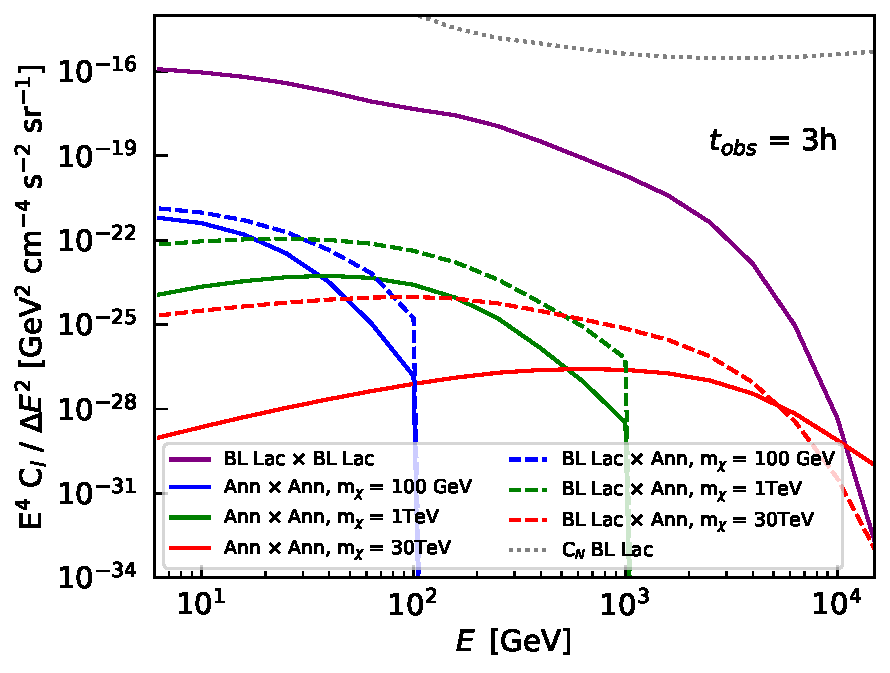
\includegraphics[width=0.45\textwidth]{figures/new_analysis/Cl_vs_E_CTA_3h.pdf}
    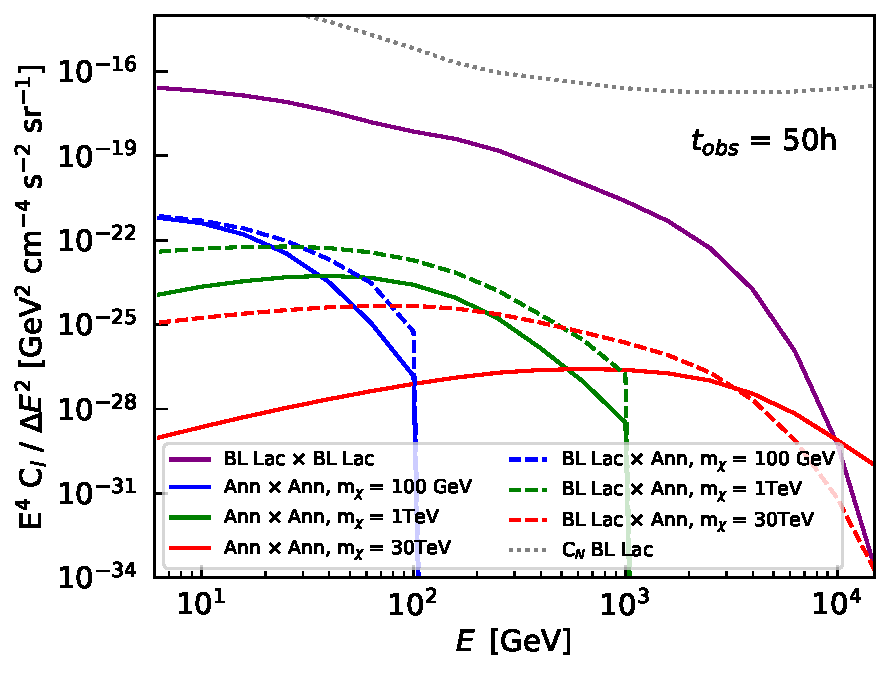
\includegraphics[width=0.45\textwidth]{figures/new_analysis/Cl_vs_E_CTA_50h.pdf}
    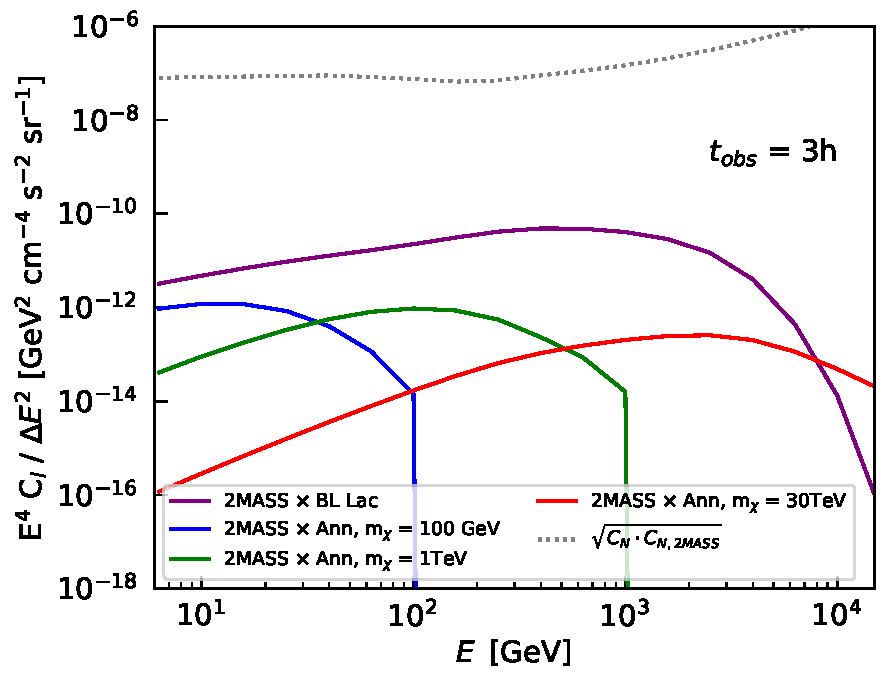
\includegraphics[width=0.45\textwidth]{figures/new_analysis/Cl_vs_E_CTA_cross_3h.pdf}
    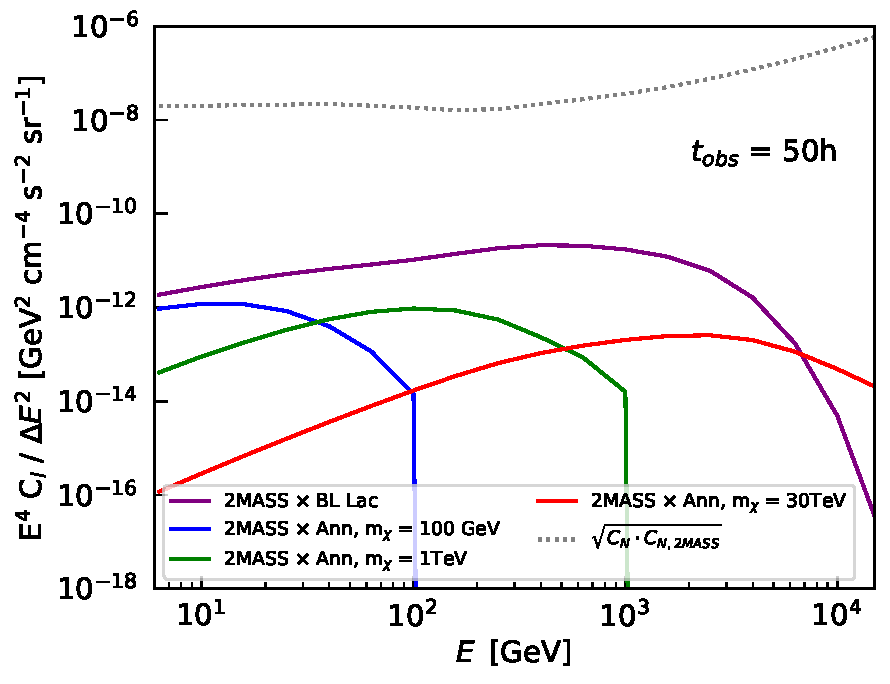
\includegraphics[width=0.45\textwidth]{figures/new_analysis/Cl_vs_E_CTA_cross_50h.pdf}
    \caption{Angular power spectra $C_\ell$ as a function of energy for $\ell=100$. The left panels correspond to 3 hours of observation, while the right panels represent 50 hours. Dark matter signals are calculated for annihilation into $b\bar{b}$, for $\langle \sigma v \rangle = 3 \times 10^{-26}$cm$^{-3}$s$^{-1}$, and three representative masses: 100 GeV, 1 TeV, and 30 TeV. The solid and dashed lines show the auto-correlation and the cross-correlation $C_\ell$ for various combinations of $\gamma$-ray emitters and galaxy catalogs, as labelled. The black dotted lines in the topmost part of the panels represent the noise level for each category: for the upper row ($\gamma$-ray auto-correlations), the noise is dominated by the photon noise of astrophysical sources, and for the lower row (cross-correlation of $\gamma$-ray with galaxies), the geometric mean of the photon and galaxy noise is shown as a representative noise level.} 
    \label{fig:Cl_vs_E}
\end{figure}


\subsection{Poisson anisotropy}
The auto-correlation angular power spectrum of blazars is dominated by the constant 1-halo term. and is therefore flat in $\ell$. It is thus convenient to define the Poisson anisotropy as the normalization of this spectrum.
\cref{fig:Cp_I2} shows the Poisson anisotropy of unresolved blazars, divided by the square of the intensity as a function of energy for 3 hours and 50 hours of observation. As expected, the anisotropy decreases with increasing observation time, since a larger fraction of the brighter sources (which contribute more significantly to the anisotropy) become resolved. Across the entire energy range, the anisotropy remains at the level of percent or below.


The same figure also shows the CTA sensitivity to the Poisson anisotropy in three energy bins. To derive this sensitivity, we adopt the same methodology used for setting the DM limits. In this case, however, the null hypothesis corresponds to pure noise, that is, the absence of any source contribution, while the alternative hypothesis assumes the presence of a source class characterized by a Poisson anisotropy. We further assume that the energy dependence of the anisotropy of this source class is proportional to $\langle I \rangle^2$, i.e., it scales with the square of the observed intensity.  As shown in the figure, the resulting sensitivity is at the level of approximately 10\%.


\begin{figure}[t!]
    \centering
    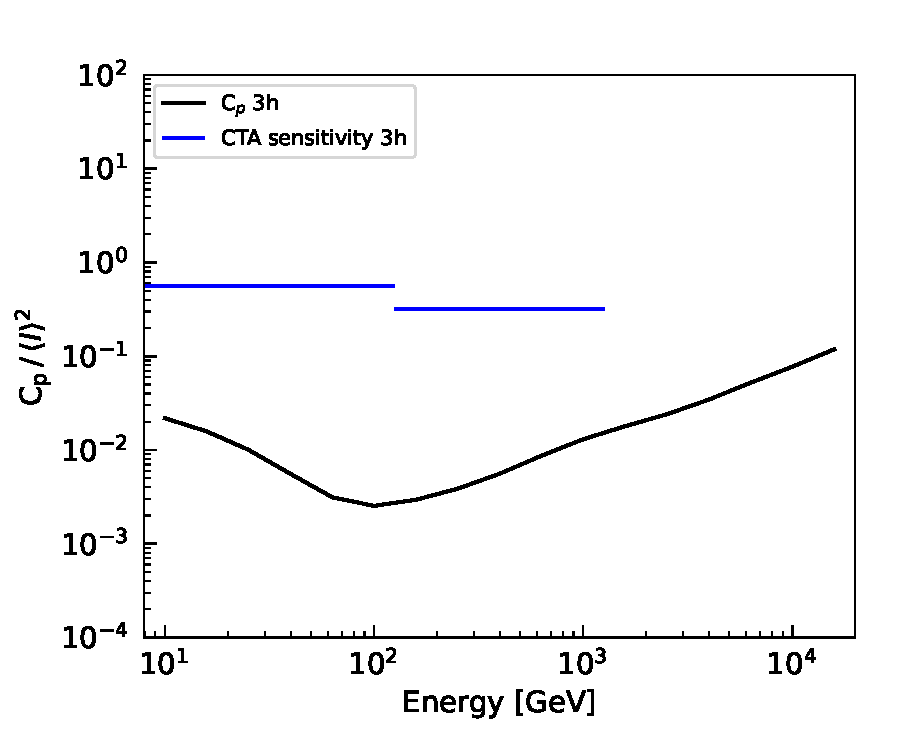
\includegraphics[width=0.45\textwidth]{figures/new_analysis/CTA_sensitivity_3h.pdf}
    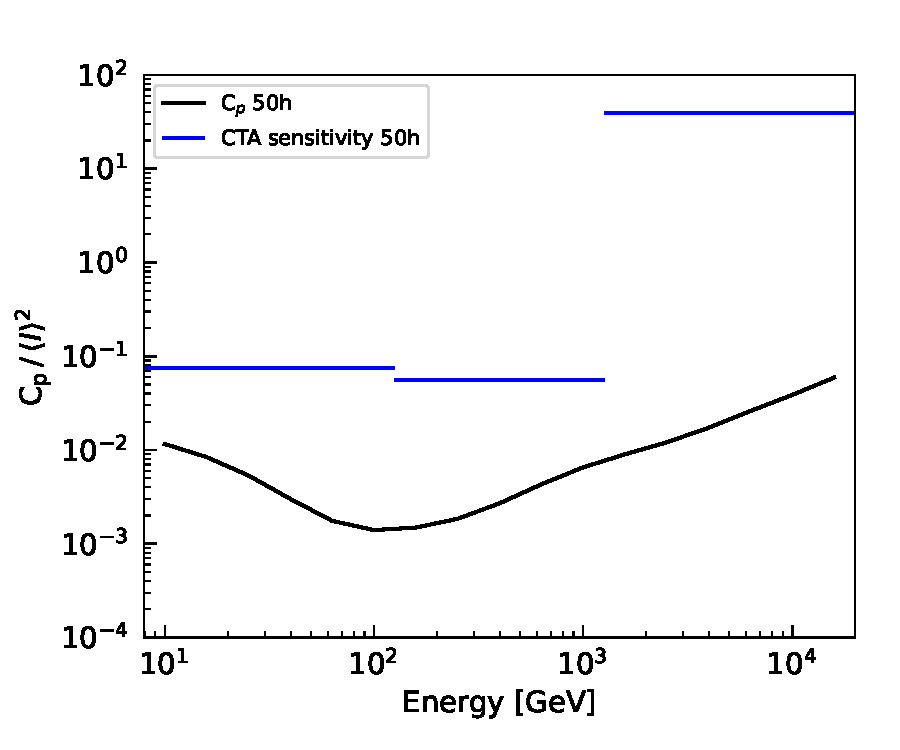
\includegraphics[width=0.45\textwidth]{figures/new_analysis/CTA_sensitivity_50h.pdf}
    \caption{CTA sensitivity to the Poisson anisotropy $C_p$ (normalized to the square of the mean $\gamma$-ray intensity) in the low, mid and high energy bins, for 3 hours (left panel) and 50 hours (right panel) of observation. The predicted sensitivity is to the expected $C_p$ from \textsl{unresolved} blazars (solid black lines). The reduced sensitivity at high energies is driven by the limited number of $\gamma$-ray events in this energy range.}
    \label{fig:Cp_I2}
\end{figure}

